\chapter{Experimental apparatus}

This chapter gives an overview of the experimental apparatus used to collect the data analyzed in this dissertation: the Large Hadron Collider (LHC) and Compact Muon Solenoid (CMS) detector. The first section reviews the design and performance of the LHC. The second section reviews the design of CMS, its component subdetectors, and data acquisition system.  

\section{Large Hadron Collider}

This section reviews the construction and original design specifications of the LHC \cite{1748-0221-3-08-S08001}, leading up to the 7-8 TeV center of mass (COM) energy collisions recorded from March 2010 to February 2013 (Run 1), the upgrades and repairs made to the LHC and its pre-accelerators during Long Shutdown 1 (LS1) from February 2013 to April 2015, and finally, the 13 TeV COM energy collisions recorded from April 2015 through 2016. 

\indent Due to budgetary and logistical concerns, the LHC is located in the repurposed Large Electron-Positron (LEP) collider tunnel, constructed in the 1980s by the European Organization for Nuclear Research (CERN), which continues to operate the LHC accelerator facilities and whose laboratory hosts the staff, scientists, and engineers running the machines and detectors associated with it. Located beneath the border of Switzerland and France near Geneva, the LEP tunnel consists of eight straight sections and eight arced sections, totalling 26.7 km, at depths varying from 45 m to 170 m. Two 2.5 km transfer tunnels connect the main LEP tunnel to the rest of the CERN complex, which includes a series of pre-accelerators that increase the energy of ionized hydrogen gas protons to 450 GeV before they are injected into the LHC. In addition to repurposing the tunnel, the underground caverns at Points 2 and 8, which were built for LEP, are used for the ALICE and LHCb experiments, the two specific purpose experiments, designed to study quark-gluon plasma in heavy ion collisions and the matter-antimatter imbalance, respectively. The facilities at Points 1 and 5, where the general-purpose ATLAS and CMS experiments are located, were built new for the LHC. 

\indent Although the length of the LEP tunnel is sufficient for the LHC, the diameter of the tunnel and the geometry of the straight and arced sections are suboptimal for a proton-proton accelerator. Since sychrotron radiation emission is not as much of a problem for a protons, the LHC would ideally have longer arced sections. The two counter circulating particle-antiparticle beams of LEP could occupy the same pipe, being curved by the same magnets, but with an inside diameter of only 3.7 m, the tunnel is too narrow to accommodate the two pipes needed for counter circulating proton-proton beams, necessitating the use of the "two-in-one" super-conducting twin bore magnet design. The LHC beam is steared by 1232 8 T, superconducting dipole twin bore magnets, which are cooled by a system of NbTi Rutherford cables to below 2 K. This technology is essential to the LHC operation, but comes at the cost of a higher sensitivity to instabilities in the operation temperature, which may cause the magnet to quench, or lose its superconductivity and current.

\indent The LHC was designed to explore physics at the EW symmetry breaking scale, with a nominal COM energy for collisions of 14 TeV, and search for rare events produced by physics beyond the SM, with a target luminosity of $10^{34} \rm{cm}^{-2} \rm{s}^{-1}$, both the highest ever produced. For a general physics process, the rate of event production is given by
\begin{equation}
N = \sigma \times L \propto \sigma \times n_b N_b^2 f_{rev} \gamma
\end{equation}
where $\sigma$ is the process cross section, $L$ is the LHC luminosity, which is proportional to $n_B$, the number of bunches per beam, $N_b^2$, the number of particles per bunch, $f_{rev}$, the beam revolution frequency, and $\gamma$, the relativistic gamma factor. Consequently, to achieve higher event rates for rare processes, both high beam intensities and high beam energies are required. To search for rare events, such as H production, the basic strategy for designing the LHC was to maximize these luminosity parameters within the budgetary, engineering, and physical limitations, of which there are many. Combining these constraints yields nominal values of 2808 bunches per beam, $1.2\times10^{11}$ protons per bunch, and a revolution frequency of 11245 turns per second. The luminosity decays over a given run with a lifetime of $\tau \approx 15$ hours, due primarily to losses in particle intensity from collisions, and must periodically be dumped and refilled with an average turnaround time of around 7 hours. The integrated luminosity is the integral of the luminosity as a function of time $L(t) = L_0 / (1+t/\tau)^2$ over a run of length $T_{run}$ given by
\begin{equation}
L_{int} = L_0 \tau (1-e^{-T_{run}/\tau})
\end{equation}
where $L_0$ is the initial luminosity. If the LHC runs for 200 days per year with a peak luminosity of $10^{34} \rm{cm}^{-2} \rm{s}^{-1}$, the maximum total integrated luminosity, or sum of the integrated luminosity of all runs is about $80 \rm{fb}^{-1}$ per year. Due to unforeseen setbacks and inefficiencies in collecting data at the detectors, the total integrated luminosity collected by the experiments is far less than the maximum, totalling around $20 \rm{fb}^{-1}$ each from ATLAS and CMS in the whole Run 1, and about $2 \rm{fb}^{-1}$ each in 2015. 

\indent The LHC machine was designed to attain a per beam energy of 7 TeV, resulting in COM collisions of 14 TeV, but an accident during beam energy ramp-up in September 2008, caused by a faulty electrical connection between two magnets and resulting in the damage of numerous magnets, resulted in delays [http://press.cern/press-releases/2008/10/cern-releases-analysis-lhc-incident]. As a result, the Run 1 beam energy was set to 3.5 TeV and later increased to 4 TeV, for 7 and 8 TeV collisions. LS1 began at the conclusion of Run 1, and consisted of a two year period of maintenance and upgrades, including consolidating and repairing interconnections between about 500 magnet cryostats, adding shielding and relocating various electronic equipment, and upgrades to the LHC's ramp up accelerators [http://home.cern/about/updates/2013/02/long-shutdown-1-exciting-times-ahead]. It was decided that Run 2 would proceed with beam energies of 6.5 TeV instead of the originally planned 7 TeV in the interest of time, since it would have taken longer to retrain the magnets to not quench below currents required for 14 TeV than it would to retrain them for 13 TeV [http://home.cern/about/engineering/restarting-lhc-why-13-tev]. Overall, the LHC has performed and continues to perform at a very high level, supplying the experiments with beam collisions within the desired luminosity ranges. 

\section{Compact Muon Solenoid}

This section reviews the design and performance of the CMS detector \cite{1748-0221-3-08-S08004}, including its general layout, subdetector systems, and trigger and data acquisition (DAQ) systems. CMS was designed to explore physics at the TeV scale, recording collisions from the LHC proton beams at their crossing place at Point 5, near Cessy, France. The detector is multi-purpose, in that it is sensitive to detecting a wide array of new physics signatures, but the primary purpose is to validate or refute the Higgs mechanism as being responsible for EW symmetry breaking. This goal was accomplished in Run 1, so Run 2 looks forward to searching for physics beyond the SM, including signatures from new symmetries such as SUSY, extra dimensions, and dark matter. Additionally, CMS is disigned to record collisions of heavy ion beams to study QCD at this energy scale. CMS is distinguished from other general purpose detectors by its high magnetic field solenoidal structure, silicon-based inner tracker, and crystal scintillator electromagnetic calorimeter. 

\indent The primary challenges in designing CMS include: accounting for the pileup of inelastic collisions on each event with sufficiently high granularity detectors and small timing resolutioin, ensuring all electronics and detector components can withstand the high radiation exposure, and triggering on the roughly $10^9$ events per second to filter out interesting events to a rate managable by the read out and computing systems. The design requirements can be summarized as follows: good muon identification and charge determination, good charged-particle momentum resolution in the inner tracker, good EM energy resolution, good diphoton, dimuon, dijet, and dielectron mass resolutions, efficient photon and lepton isolation, and good MET measurement. All of these requirements will be addressed in the remainder of this chapter.

\indent With an overall length of 21.6 m and an outer diameter of 14.6 m, the cylindrical shape of CMS is divided into two regions, the barrel and endcaps, with the coordinate system centered at the collision point near the center of the cylinder. The standard coordinate definitions have the x-axis pointing inward toward the center of the LHC, the y-axis pointing upward, and the z-axis in the beam direction in a right-handed manner. The polar coordinates $r$ and $\phi$ are measured in the x-y plane, transverse to the beam, where the transverse momentum quantity $p_T$ is defined. The missing energy $E_T^{miss}$ is defined as the imbalance in measured $p_T$. The polar angle $\theta$ is measured from the z-axis. A convenient coordinate for relativistic measurements is the pseudorapidity, defined as $\eta = -\ln{\tan(\theta/2)}$. 

\begin{figure}[tbh]
\centering
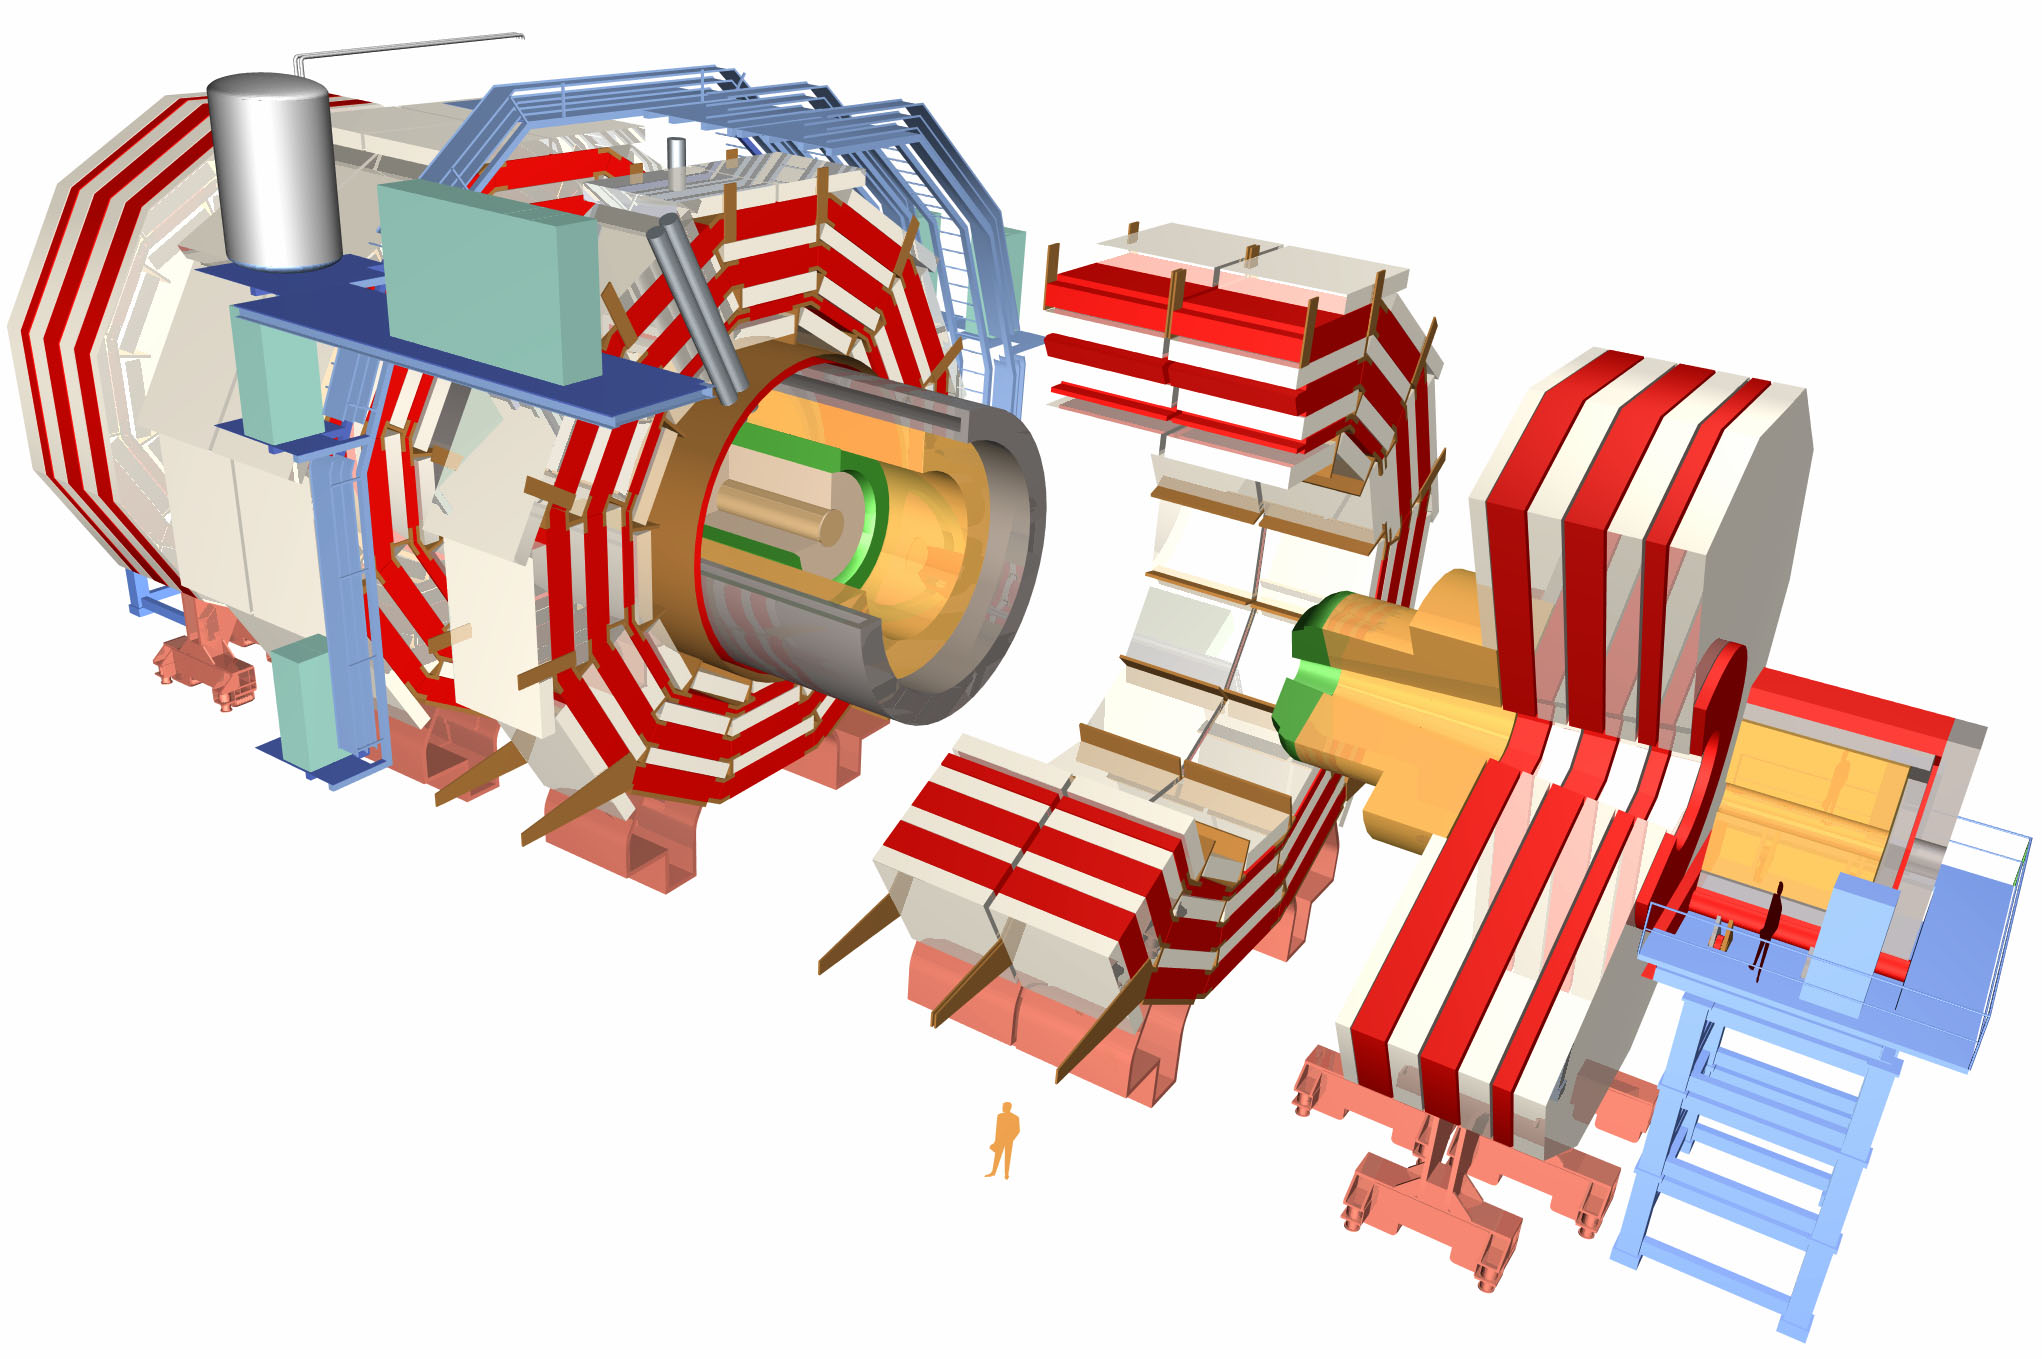
\includegraphics[width=6in]{figures/cms.jpg}
\caption{Deconstructed view of the CMS subdetectors, with human figure for scale. From inside to out, the colored segments correspond to the following systems: light brown is the pixel tracker, cream is the strip tracker, green is the ECAL, orange is the HCAL, grey is the solenoid, red is the yoke with white muon chambers. }
\label{fig:cms}
\end{figure}

\indent The dominant feature of CMS is the superconducting solenoid, 13 m long and 6 m in diameter, supplying a field of 4 T required to bend charged particles at the energies produced in up to 14 TeV collisions for the momentum and charge measurements. Within and surrounding the solenoid is a series of layered detectors and support structure, a cutout of which is shown in Figure~\ref{fig:cms}. At the center of CMS, surrounding the beam interaction point, is the inner tracker, a combination of 10 layers of silicon microstrip detectors and 3 layers of silicon pixel detectors, which provide the required granularity for high occupancy collisions. The next layer, still within the solenoid bore, contains the calorimeters, first the electromagnetic calorimeter (ECAL), surrounded by the hadronic calorimeter (HCAL). The ECAL uses avalanche photodiodes in the barrel and vacuum photodiodes in the endcaps to read out scintillation light from lead tungstate crystals, produced by charged particle interactions. The HCAL in the barrel uses hybrid photodetectors to read scintillation light from hadronic interactions with the brass/scintillator detector material. The scintillation light is carried to the photodetectors with clear fibres, from wavelength shifting fibres embedded in the scintillator material. The various endcap HCAL systems ensure full coverage for measuring the missing energy. Finally, muon detecting stations are incorporated into and surround the solenoid support structure where the return field is present, including aluminum drift tubes (DTs) in the barrel and cathode strip chambers (CSCs) in the endcaps. The subdetector systems of CMS are covered in greater detail in the remainder of this chapter. 

\subsection{Tracking detectors}

The inner tracking detectors of CMS, supported by a 5.30 m long tube with an inner diameter of 2.38 m suspended from the HCAL barrel, contain 1440 pixel and 15148 strip detector modules, composing the pixel detector and silicon strip tracker, respectively. The detectors are responsible for measuring the trajectories of charged particles, essential to measuring the momenta of particles with energy $>$ 1 GeV in the range $|\eta|<2.5$, and reconstructing secondary vertices and impact parameters, needed to ID heavy flavor particles. Being closest to the beam interaction point (IP), the tracking detectors are subjected to the highest radiation doses, and their material may interfere with the trajectories of primary particles through multiple scattering, bremsstrahlung, photon conversion, or nuclear interactions, necessitating the use of silicon technology. Additionally, due to the high particle flux of around 1000 particles per 25 ns bunch crossing, the detectors must have high granularity to resolve the trajectories of particles reliably, and fast readout times to reduce occupancy from high flux and pileup conditions. 

\indent The detector modules of the tracking detector are shown schematically in Figure~\ref{fig:tracker}. The innermost section, labeled PIXEL, is the pixel detector, composed of 66 million 100 $\mu$m $\times$ 150 $\mu$m pixels on modules layered in three barrels at radii 4.4, 7.3, and 10.2 cm and two disks on each end at $z = \pm34.5, \pm46.5$ cm. A deconstructed barrel pixel module is shown in Figure~\ref{fig:pixmodule}, with the sensor bump-bonded onto read out chips (ROCs) controlled and powered by high-density-interconnect (HDI) boards. When a charged particle passes through a pixel sensor, consisting of n-type pixels implanted on a high-resistance n-type substrate, charge carriers are induced in the conduction band of the substrate. These charge carriers then drift in the 4 T magnetic field to the nearby pixels (called charge sharing), where an analog signal is read out, amplified, and digitized by the ROC. The endcap pixel modules have a similar construction, but with different pixel sensor geometries, called plaquettes. The pixel detector has a resolution of 10-40 $\mu$m, sufficient for the imposed design requirements. 

\begin{figure}[tbh]
\centering
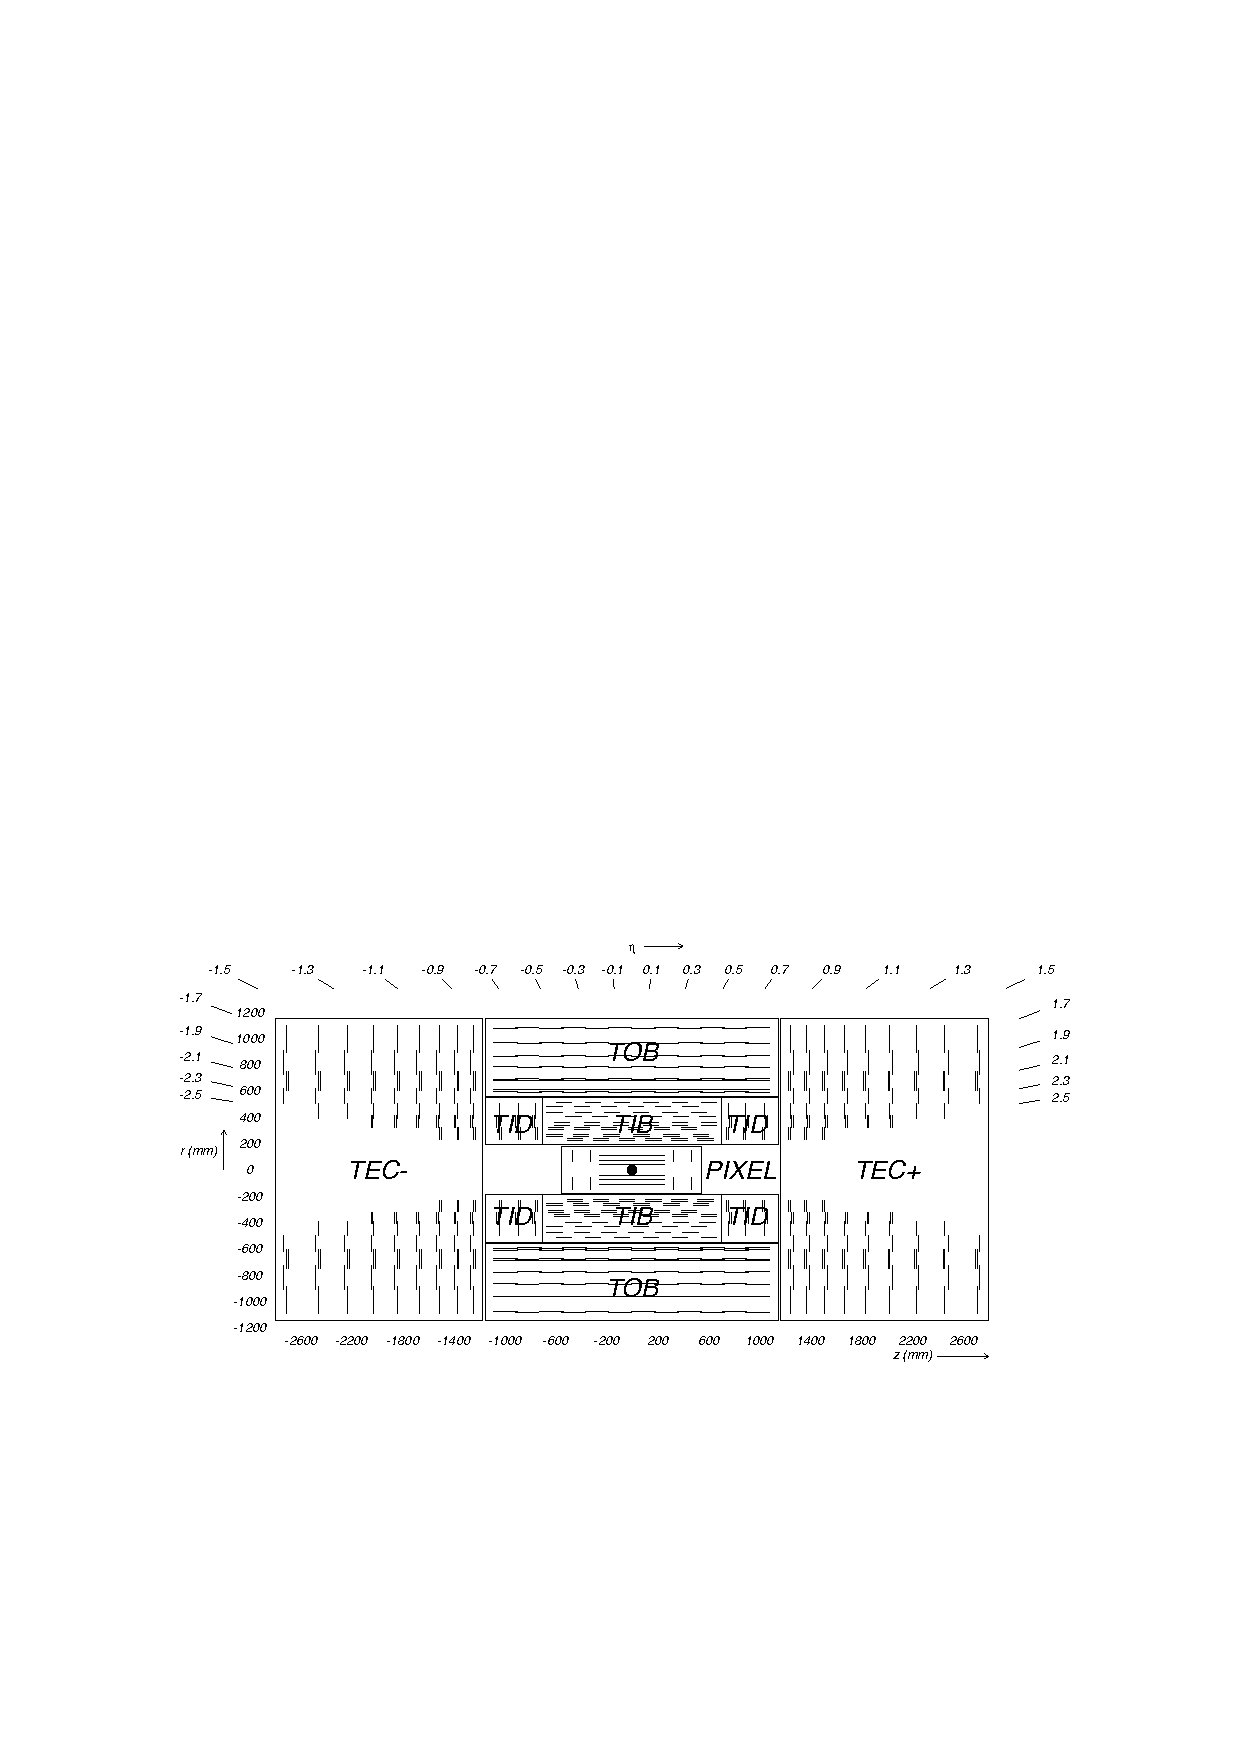
\includegraphics[width=6in]{figures/tracker.pdf}
\caption{Schematic diagram of tracking detectors with radial distance of modules (shown as black lines) from center on the left axis, z-dimension on the bottom axis, and $\eta$ accross the top.}
\label{fig:tracker}
\end{figure}

\begin{figure}[tbh]
\centering
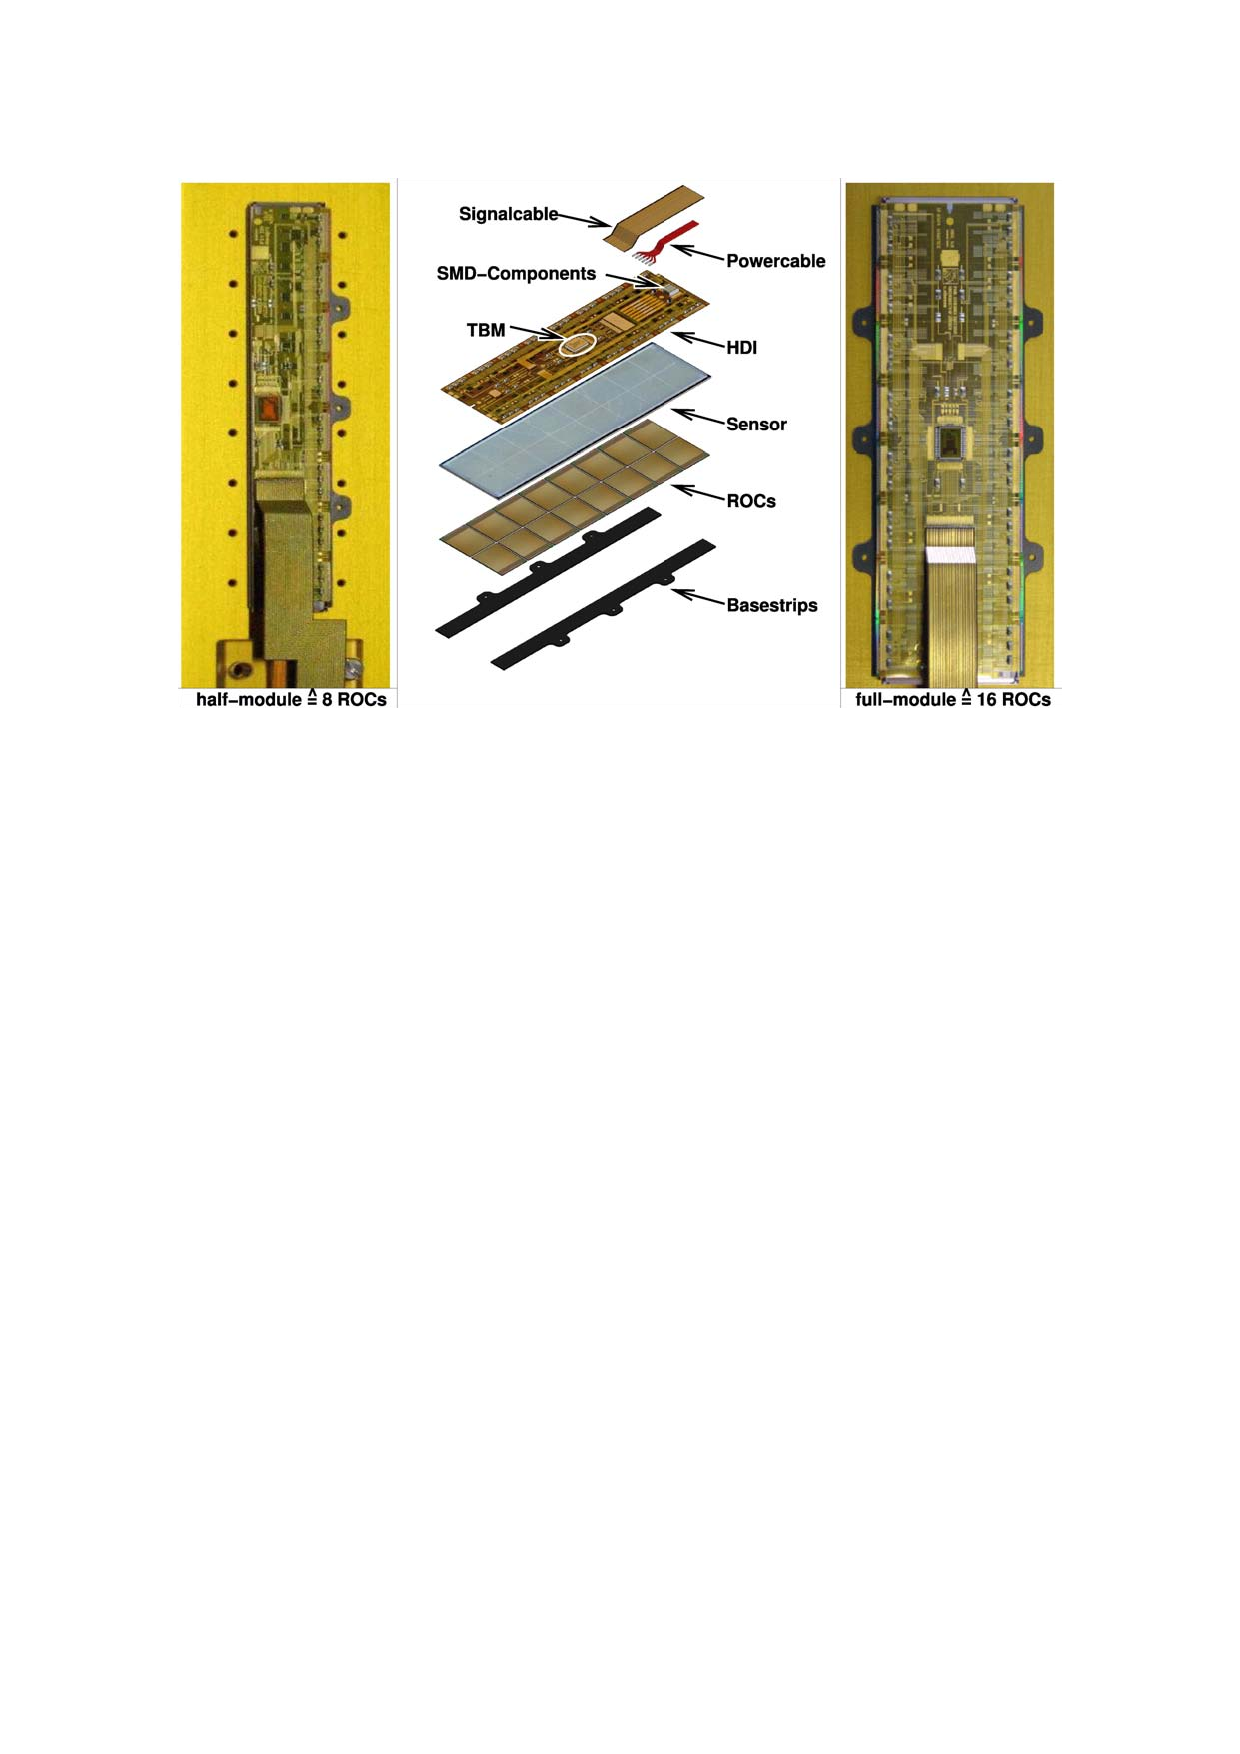
\includegraphics[width=5in]{figures/pixelmodule.pdf}
\caption{Deconstructed barrel pixel module showing module components.}
\label{fig:pixmodule}
\end{figure}

\indent The remaining modules of the pixel detector form the strip tracker. These are divided into the following sections: 

\subsection{Electromagnetic calorimeter}

\subsection{Hadronic calorimeter}

\subsection{Muon detectors}

\subsection{Trigger system}

